\section{Auswertung}
\label{sec:evaluation}
Ausgleichsrechnungen mit den dazugehörigen Fehlern werden mit dem \texttt{python}-Paket \texttt{SciPy} \cite{scipy} erstellt, weitere Fehler werden mit dem \texttt{python}-Paket \texttt{uncertainties} \cite{uncertain} berechnet, welches eine automatische Gauß'sche Fehlerfortpflanzung bereitstellt.

\subsection{Frequenzgang eines gegengekoppelten Verst\"{a}rkers}
\label{Frequenzgang}
Die Frequenzabhängigkeit des Linearverstärkers wird untersucht, indem die Verstärkung bei verschiedenen Frequenzen über mehrere Zehnerpotenzen gemessen wird. Dies wird für vier verschiedene Kombinationen von Widerständen durchgeführt. Eine doppelt-logarithmische Darstellung der Frequenzgänge ist in \autoref{fig:a} gezeigt. Die durchgezogene Linie stellt dabei jeweils den linearen Fit der Form
\begin{equation}
	\log_{10} {V_0}^\prime = A \cdot \log_{10} \frac{\nu}{\SI{1}{\hertz}} + B
	\label{linear_fit}
\end{equation}
an den abfallenden Teil bei hohen Frequenzen dar, wobei der Plateauwert ${V_0}^\prime = U_\text{A} / U_\text{E}$ der Mittelwert aus dem Quotienten aus Ausgangs- und Eingangsspannung für Frequenzen $\nu < \SI{10}{\hertz}$ ist. In \autoref{tab:a} werden die verwendeten Widerstände, die daraus resultierenden Fitparameter und die Grenzfrequenzen $\nu_\text{G}$ -- also die Frequenz, bei der die Verstärkung auf $V'/\sqrt{2}$ abgefallen ist -- zusammengefasst. Die Grenzfrequenz wird über
\begin{equation*}
	\nu_\text{G} = 10^{\left[\log_{10}\left({V_0}^\prime/\sqrt{2}\right) - B\right] / A}
\end{equation*}
berechnet. Das Verstärkung-Bandbreite-Produkt $\nu_\text{G}{V_0}^\prime$ ist ebenfalls eingetragen. Der Mittelwert des Verstärkung-Bandbreite-Produkts der vier gemessenen Widerstandskombinationen ist
\begin{equation*}
	\bar{\nu_\text{G}{V_0}^\prime} = \SI{833 \pm 37}{\hertz},
\end{equation*}
die Abweichungen der einzelnen Werte vom Mittelwert liegen zwischen 1.6\% und 6.6\%. Mit \autoref{effVerstaerkung} kann aus ${V_0}^\prime$ und den beiden Widerständen $R_1$ und $R_\text{N}$ die Leerlaufverstärkung $V$ mit
\begin{equation}
	V = \frac{R_\text{N} + R_1}{\frac{R_\text{N}}{{V_0}^\prime} - R_1}
\end{equation}
abgeschätzt werden. Die entsprechenden Werte sind ebenfalls in \autoref{tab:a} eingetragen.\par
In \autoref{scope_234} werden beispielhaft ein Sinussignal als Eingangssignal (in grün) und das verstärkte Ausgangssignal (in gelb) als Oszilloskopaufnahme gezeigt. Da das Eingangssignal auf den invertierenden Eingang des Operationsverstärkers gegeben wird, beträgt die Phase zwischen Ein- und Ausgangssignal nahezu $180^\circ$, das Eingangssignal wird bei einer Frequenz von $\SI{99.90}{\hertz}$ von $\SI{197}{\milli\volt}$ um einen Faktor von fast 5 auf $\SI{970}{\milli\volt}$ verstärkt.
\begin{figure}[h]
	\centering
	\begin{subfigure}[t]{0.5\textwidth}
		\centering
		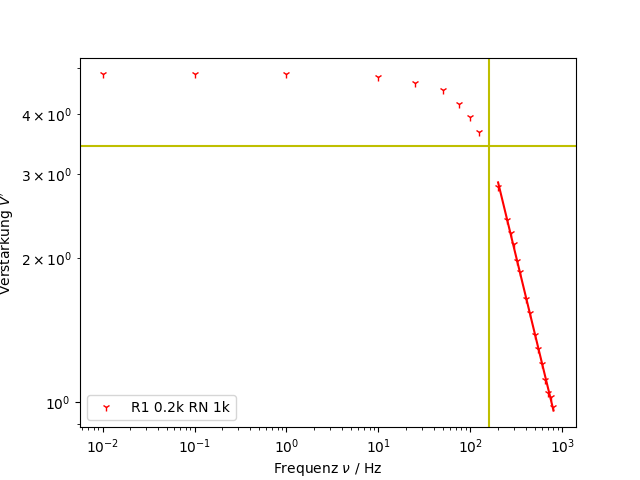
\includegraphics[width=\textwidth]{img/a_R1_0-2k_RN_1k.png}
	\end{subfigure}%
	~
	\begin{subfigure}[t]{0.5\textwidth}
		\centering
		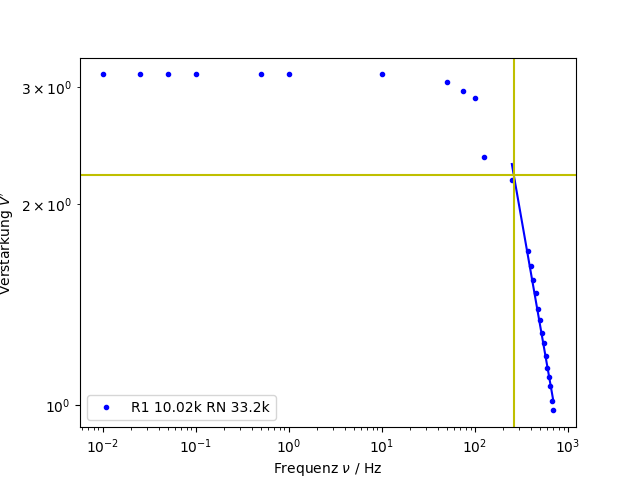
\includegraphics[width=\textwidth]{img/a_R1_10-02k_RN_33-2k.png}
	\end{subfigure}
	\\
	\begin{subfigure}[t]{0.5\textwidth}
		\centering
		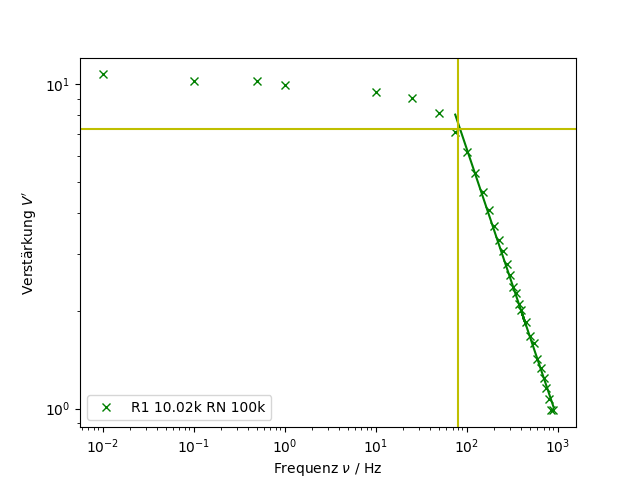
\includegraphics[width=\textwidth]{img/a_R1_10-02k_RN_100k.png}
	\end{subfigure}%
	~
	\begin{subfigure}[t]{0.5\textwidth}
		\centering
		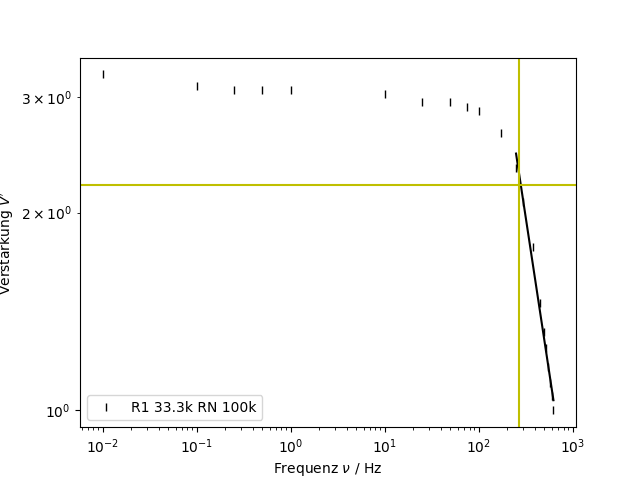
\includegraphics[width=\textwidth]{img/a_R1_33-3k_RN_100k.png}
	\end{subfigure}
	\caption{Frequenzgang eines gegengekoppelten Verstärkers - bei kleinen Frequenzen ist die Verstärkung in etwa konstant, nimmt dann aber mit größer werdenden Frequenzen in der doppelt-logarithmischen Darstellung linear ab. Für die Berechnung der Verstärkung werden Frequenzen $\nu < \SI{10}{\hertz}$ genutzt.}
	\label{fig:a}
\end{figure}
\begin{table}[h]
	\caption{Zusammenfassung der Messergebnisse des Linearverstärkers.}
	\label{tab:a}
	\centering
	\begin{tabular}{ccccccccc}
		$R_1/\si{\kilo\ohm}$	&	$R_\text{N}/\si{\kilo\ohm}$	&	A	&	B	&	${V_0}^\prime$	&	$R_{N}/R_1$	&	$\nu_\text{G}/\si{\hertz}$	&	$\nu_\text{G}{V_0}^\prime/\si{\hertz}$	&	$V$	\\ \toprule
		10.02	&	100.0	&	-0.83\pm0.01	&	2.47\pm0.03	&	10.20 	&	9.98	&	80.74	&	862	&	-165.33\\
		10.02	&	33.2	&	-0.80\pm0.02	&	2.27\pm0.06	&	3.13 	&	3.31	&	262.07	&	820	&	226.91\\
		0.20	&	1.0	&	-0.79\pm0.01	&	2.28\pm0.03	&	4.85 	&	5.00	&	160.60	&	778	&	194.00\\
		33.30	&	100.0	&	-0.94\pm0.04	&	2.70\pm0.10	&	3.127	&	3.00	&	269.00	&	873	&	-52.67\\
	\end{tabular}
\end{table}
\begin{figure}[h]
	\centering
	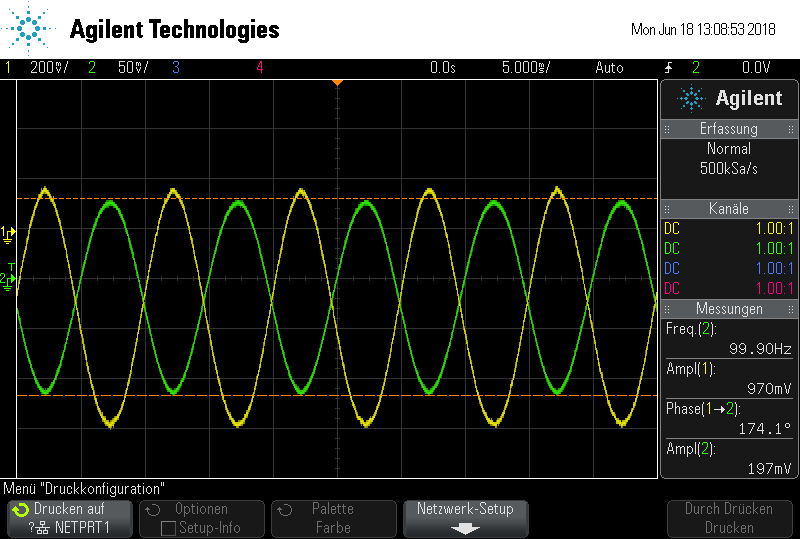
\includegraphics[width=\textwidth]{usb/scope_234.png}
	\caption{Im Plateaubereich bei kleinen Frequenzen ist die Verstärkung in etwa konstant, die Phase des Ausgangssignals ist gegenüber dem Eingangssignal um nahezu $180^\circ$ gedreht.}
	\label{scope_234}
\end{figure}

\FloatBarrier

\subsubsection{Beziehung zwischen Frequenz und Phase}

Die Phase zwischen Eingangs- und Ausgangsspannung in Abhängigkeit von der Frequenz hat einen ähnlichen Verlauf, wie die Verstärkung, sie ist in \autoref{Phasenbeziehung} zu sehen. Zunächst ist die Phase konstant und nahezu $180^\circ$. Nach einer Frequenz von \SI{10}{\hertz} fällt die die Phase ab. Das ist mit dem Einsetzen des Tiefpass-Verhaltens des Operationsverstärkers zu erklären; bei hohen Frequenzen sinkt die Verstärkung auf 1 ab. Die Übertragungsfunktion eines Tiefpasses verläuft gemäß
\begin{equation}
	H(\omega) = \frac{1}{1 + i\frac{\omega}{\omega_\text{g}}},
\end{equation}
das heißt, je näher die Frequenz gegen die Grenzfrequenz $\omega_\text{g}$ geht, desto größer ist die Phasendrehung zunächst, nähert sich dann aber einem Sättigungswert an. Der Phasengang eines Operationsverstärkers folgt nicht dem Verlauf eines reinen Tiefpasses, sondern ist abhängig vom inneren Aufbau, tendentiell lässt sich aber sagen, dass auch hier die Phasendrehung mit größerer Frequenz steigt.

\begin{figure}[h]
	\centering
	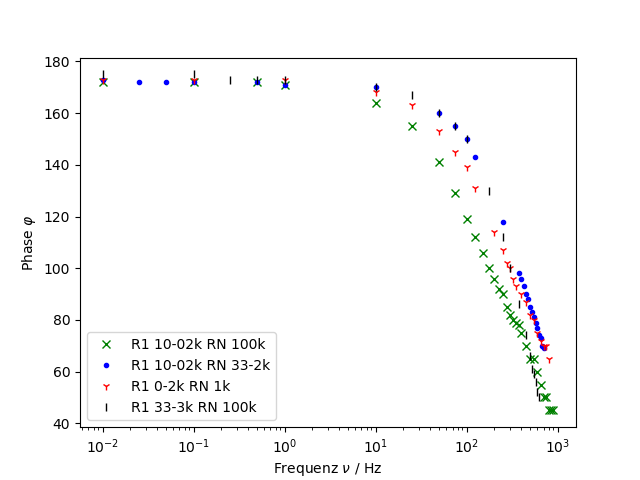
\includegraphics[width=\textwidth]{img/j.png}
	\caption{Bis zu einer Frequenz von \SI{10}{\hertz} ist die Phase relativ konstant bei knapp $180^\circ$, danach fällt sie in der halblogarithmischen Darstellung nahezu linear ab.}
	\label{Phasenbeziehung}
\end{figure}

\FloatBarrier

\subsection{Umkehr-Integrator und Differentiator}

\subsubsection{Umkehr-Integrator}

Der Fit der Form
\begin{equation}
	\log_{10} \frac{U_\text{A}}{U_\text{E}} = A \cdot \log_{10} \frac{\nu}{\SI{1}{\hertz}} + B
\end{equation}
liefert die Parameter
\begin{equation}
	A = -0.93 \pm 0.01 \quad \text{und} \quad B = -1.496 \pm 0.003,
\end{equation}
die Messwerte mit der linearen Ausgleichsgeraden sind in \autoref{fig:d} zu sehen. Die ersten drei Messwerte werden dabei nicht genutzt, da die Phase nicht mit dem gewünschten Wert von $\approx \SI{90}{\degree}$ übereinstimmt (siehe dazu \autoref{tab:d}).
\begin{figure}[h]
	\centering
	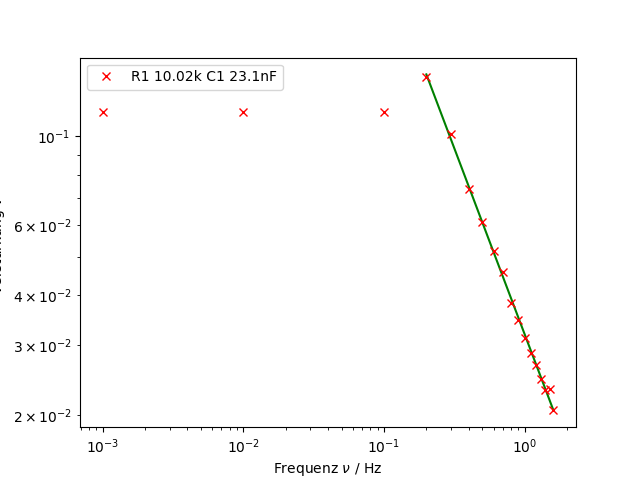
\includegraphics[width=\textwidth]{img/d.png}
	\caption{In dem dargestellten Frequenzbereich fällt die auf die Eingangsspannung normierte Ausgangsspannung nach dem Umkehr-Integrator in der doppelt-logarithmischen Darstellung linear mit der Frequenz ab; die ersten drei Messwerte werden für die lineare Ausgleichsrechnung nicht genutzt.}
	\label{fig:d}
\end{figure}
In \autoref{scope_242}, \autoref{scope_243} und \autoref{scope_244} ist jeweils zu sehen, welches Ausgangssignal der Umkehr-Integrator liefert, wenn ein Sinus-, Rechteck- bzw. Dreiecksignal auf den Eingang gegeben wird.\begin{figure}[h]
	\centering
	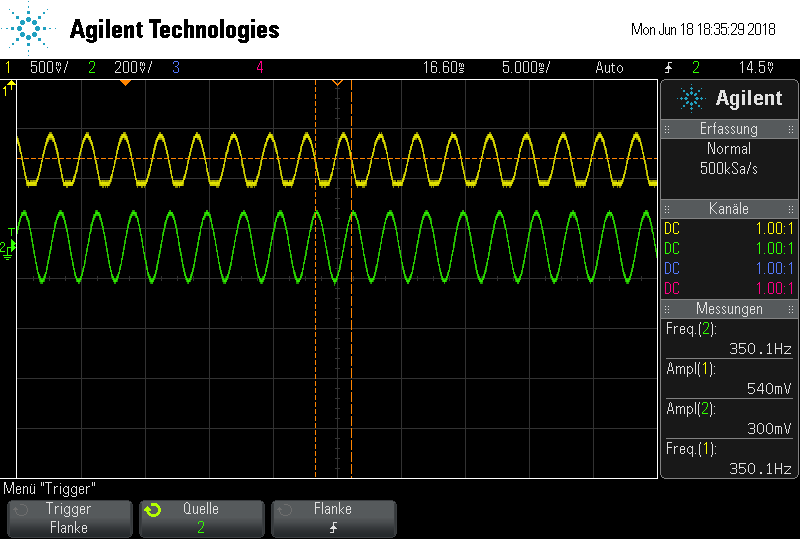
\includegraphics[width=\textwidth]{usb/scope_242.png}
	\caption{Der Umkehr-Integrator liefert bei einem Sinussignal einen Cosinus mit einer Phasendrehung von $90^\circ$ gegenüber dem Eingangssignal.}
	\label{scope_242}
\end{figure}
\begin{figure}[h]
	\centering
	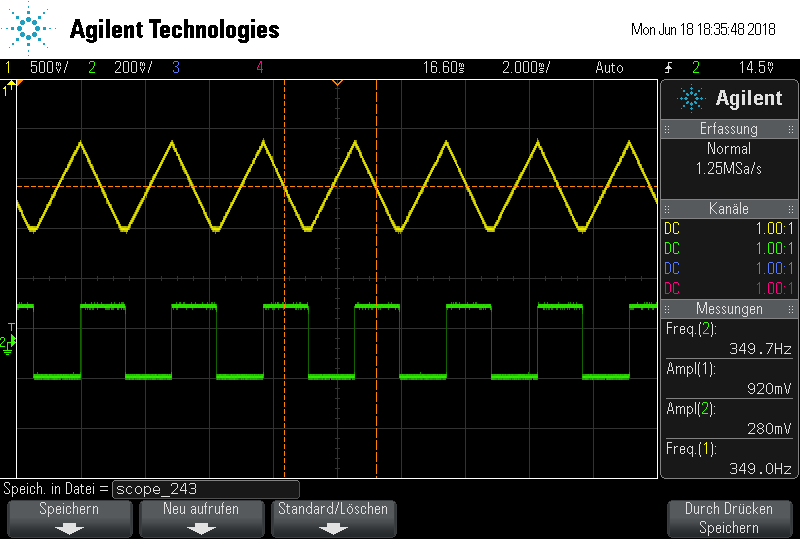
\includegraphics[width=\textwidth]{usb/scope_243.png}
	\caption{Der Umkehr-Integrator liefert bei einem Rechtecksignal ein Dreiecksignal.}
	\label{scope_243}
\end{figure}
\begin{figure}[h]
	\centering
	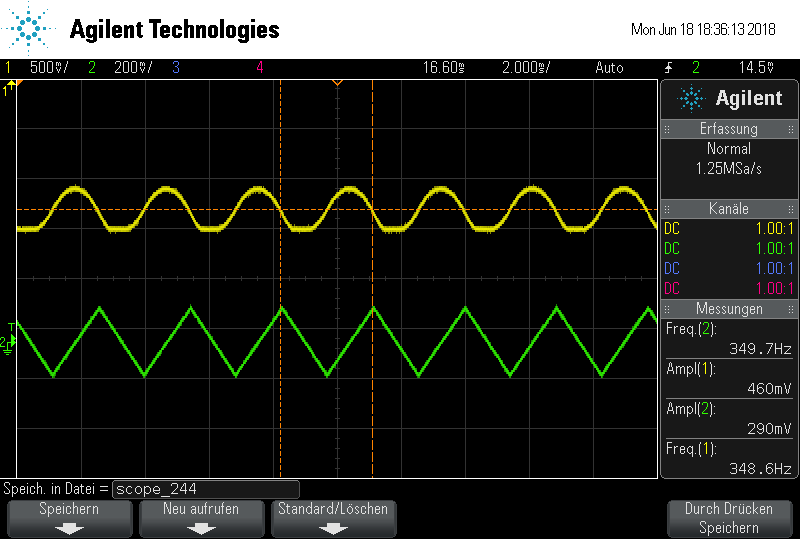
\includegraphics[width=\textwidth]{usb/scope_244.png}
	\caption{Der Umkehr-Integrator liefert bei einem Dreiecksignal näherungsweise eine Abfolge von Parabeln.}
	\label{scope_244}
\end{figure}

\FloatBarrier

\subsubsection{Umkehr-Differentiator}

Der Fit der Form
\begin{equation}
	\log_{10} \frac{U_\text{A}}{U_\text{E}} = A \cdot \log_{10} \frac{\nu}{\SI{1}{\hertz}} + B
\end{equation}
liefert die Parameter
\begin{equation}
	A = 0.73 \pm 0.01 \quad \text{und} \quad -1.381 \pm 0.002,
\end{equation}
die Messwerte mit der linearen Ausgleichsgeraden sind in \autoref{fig:e} zu sehen.
\begin{figure}[h]
	\centering
	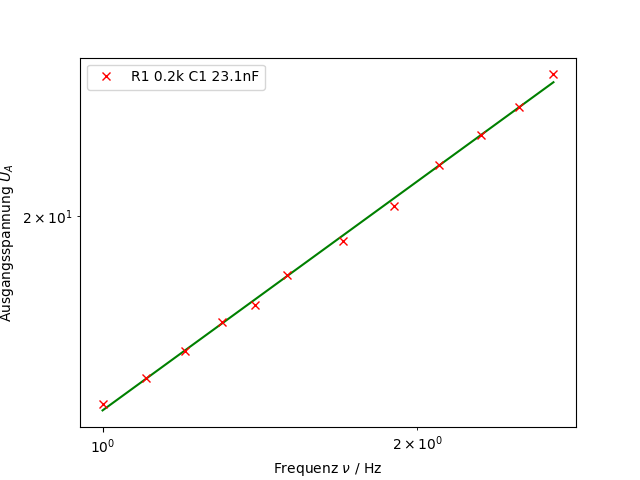
\includegraphics[width=\textwidth]{img/e.png}
	\caption{In dem dargestellten Frequenzbereich steigt die auf die Eingangsspannung normierte Ausgangsspannung nach dem Umkehr-Differentiator in der doppelt-logarithmischen Darstellung linear mit der Frequenz an.}
	\label{fig:e}
\end{figure}
In \autoref{scope_245}, \autoref{scope_246} und \autoref{scope_247} ist jeweils zu sehen, welches Ausgangssignal der Umkehr-Integrator liefert, wenn ein Sinus-, Rechteck- bzw. Dreiecksignal auf den Eingang gegeben wird.
\begin{figure}[h]
	\centering
	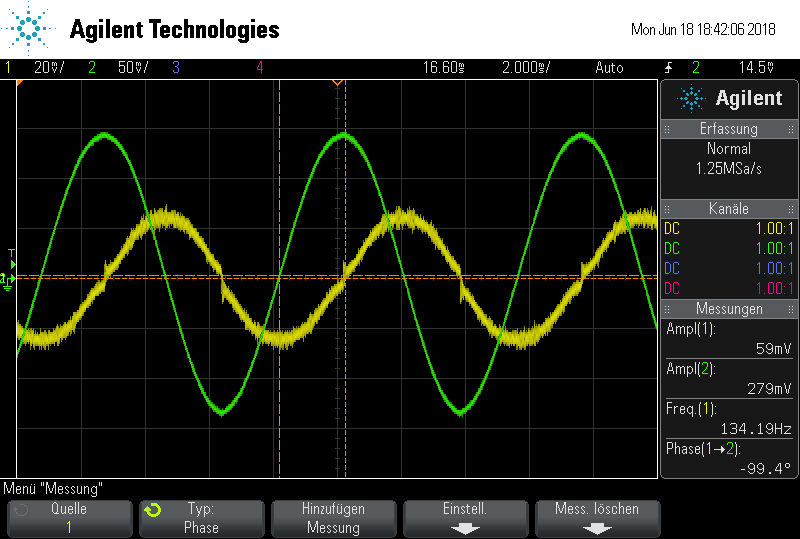
\includegraphics[width=\textwidth]{usb/scope_245.png}
	\caption{Der Umkehr-Differentiator liefert bei einem Sinussignal einen Cosinus mit einer Phasendrehung von $90^\circ$ gegenüber dem Eingangssignal.}
	\label{scope_245}
\end{figure}
\begin{figure}[h]
	\centering
	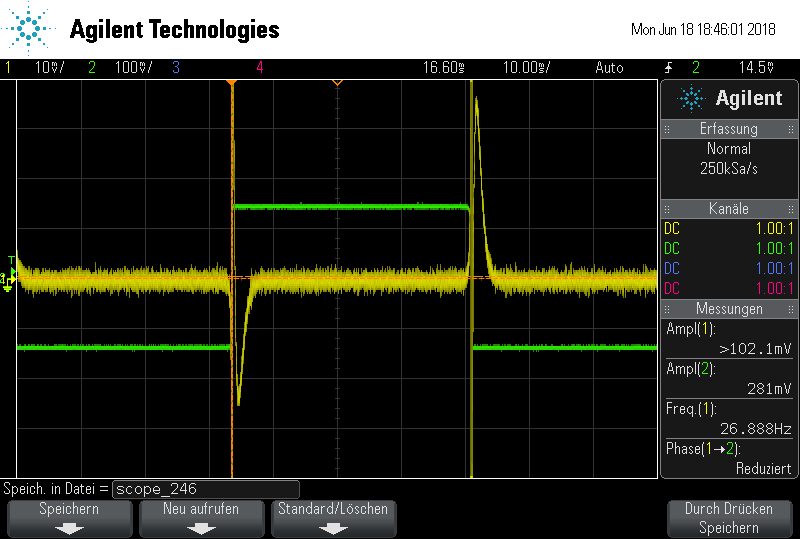
\includegraphics[width=\textwidth]{usb/scope_246.png}
	\caption{Der Umkehr-Differentiator liefert bei einem Rechtecksignal eine Abfolge von Deltapeaks.}
	\label{scope_246}
\end{figure}
\begin{figure}[h]
	\centering
	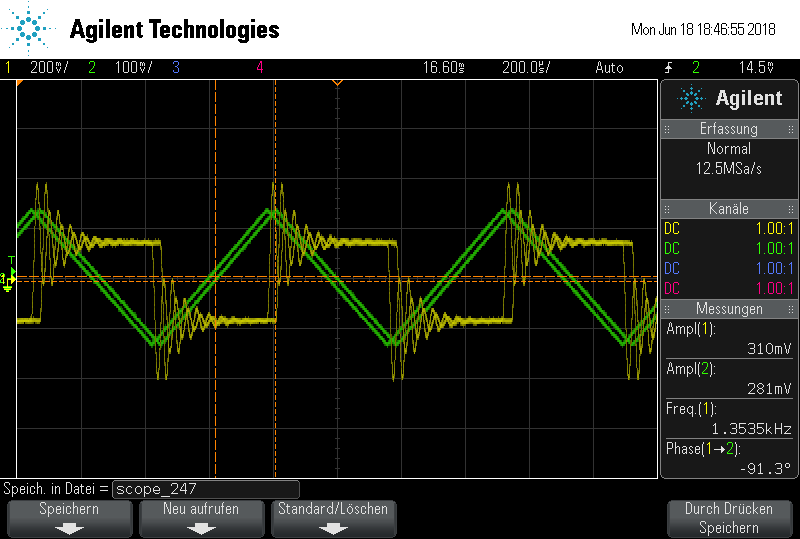
\includegraphics[width=\textwidth]{usb/scope_247.png}
	\caption{Der Umkehr-Differentiator liefert bei einem Dreiecksignal ein Rechtecksignal.}
	\label{scope_247}
\end{figure}

\FloatBarrier

\subsection{Schmitt-Trigger}

Mit Hilfe der Schaltung in \autoref{abb:sch} wird ein Schmitt-Trigger implementiert. Es werden die Widerstände $R_\text{P} = \SI{10}{\kilo\ohm}$ und $R_\text{1} = \SI{0.2}{\kilo\ohm}$ bei einer Frequenz von $f = \SI{1}{\kilo\hertz}$ benutzt, die doppelte Betriebsspannung ist $2U_\text{B} = \SI{7.86}{\volt}$. Mit
\begin{equation}
	U_\text{trig,theo} = U_\text{B} \cdot \frac{R_1}{R_\text{P}}
\end{equation}
wird die theoretische Triggerschwelle als
\begin{equation*}
	U_\text{trig,theo} \approx \SI{\pm 78.6}{\milli\volt}
\end{equation*}
berechnet. Die gemessenen Wertefür den oberen bzw. unteren Triggerpunkt sind
\begin{equation*}
	U_\text{trig,exp} \approx \SI{82}{\milli\volt} \quad \text{und} \quad U_\text{trig,exp} \approx \SI{-95}{\milli\volt}.
\end{equation*}
Die Abweichung zwischen theoretischem und experimentellen Wert beträgt 4.3\% bzw. 20.9\%. Die entsprechende Oszilloskopaufnahme ist in \autoref{scope_237} zu sehen.
\begin{figure}[h]
	\centering
	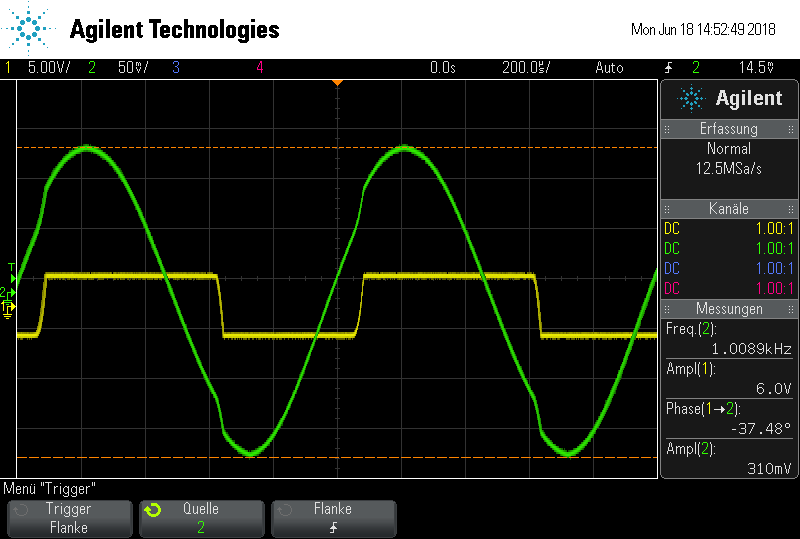
\includegraphics[width=\textwidth]{usb/scope_237.png}
	\caption{Durch den Schmitt-Trigger wird ein Ausgangssignal generiert, sobald das Eingangssignal die Triggerschwelle überschritten hat.}
	\label{scope_237}
\end{figure}

\FloatBarrier

\subsection{Dreiecksgenerator}

Zunächst wird eine Sinusschwingung mit der Frequenz $f_\text{Sinus} = \SI{1}{\kilo\hertz}$ als Anstoß-Signal auf einen Schmitt-Trigger gegeben. Bei einer Triggerschwelle von $U_\text{E} = \SI{165}{\milli\volt}$ entsteht ein Rechtecksignal. Ein Integrator macht daraus ein Dreiecksignal, welches bei der Triggerschwelle eine Amplitude von $U_\text{Dreieck} = \SI{2.09}{\volt}$ und ebenfalls eine Frequenz von $f_\text{Dreieck} = \SI{1}{\kilo\hertz}$ hat. Da das Signal auf dem invertierenden Eingang liegt, hat der positive kontante Wert eine linear abfallende Spannung zur Folge, eine konstante negative Spannung eine hingegen eine ansteigende Spannung. \autoref{scope_239} zeigt das Dreiecksignal bei einer höheren Eingangs- und Ausgangsspannung. Aufgrund eines Fehlers in der Durchführung dieses Versuchsteils, unterscheiden sich die Ergebnisse deutlich von den theoretisch vorhergesagten Werten. Anhang von \autoref{frequenz} wird die theoretisch erwartete Frequenz des Rechteck- und Dreiecksignals zu
\begin{equation*}
	f_\text{theo} = \SI{54.113}{\kilo\hertz}
\end{equation*}
bestimmt. Die Werte der Widerstände und des Kondensators sind $R = \SI{10}{\kilo\ohm}$, $R_\text{P} = \SI{10}{\kilo\ohm}$, $R_1 = \SI{0.2}{\kilo\ohm}$ und $C = \SI{23.1}{\nano\farad}$. Wegen der falschen Durchführung ist der theoretische Wert 54-mal größer als die gemessene Frequenz. Nach \autoref{differenz} ist die theoretische Amplitude der Rechteckspannung mit $U_\text{B} = \SI{3.94}{\volt}$
\begin{equation*}
	U_\text{theo} = \SI{157.6}{\milli\volt}\, ,
\end{equation*}
diese wurde allerdings durch einen Fehler in der Durchführung nicht gemessen, sodass kein Vergleichswert existiert.
\begin{figure}[h]
	\centering
	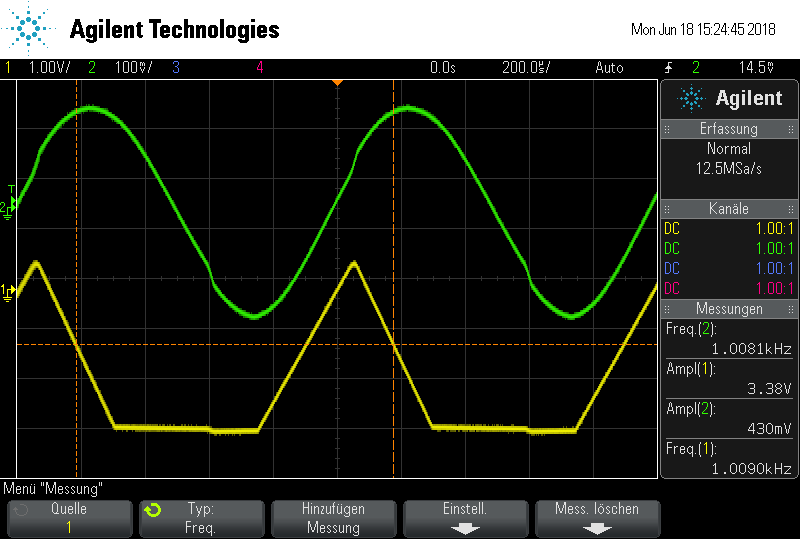
\includegraphics[width=\textwidth]{usb/scope_239.png}
	\caption{Mit Hilfe des Schmitt-Triggers wird aus einer Sinusschwingung (grün) zunächst ein Rechtecksignal generiert, aus welchem dann mit einem Integrator ein Dreiecksignal (gelb) gemacht wird.}
	\label{scope_239}
\end{figure}

\FloatBarrier

\subsection{Ged\"{a}mpften und unged\"{a}mpfte Schwingung}

In \autoref{scope_241} ist die ungedämpfte Schwingung mit einer charakteristischen Frequenz von $f = \SI{758}{\hertz}$ dargestellt. Die Amplitude bleibt nahezu konstant.\par
Theoretisch ergibt sich bei der gedämpften Schingung nach $f = 1 / 2\pi RC$ und $\tau = 20RC$ eine Schwingungsfrequenz von
\begin{equation*}
	f_\text{theo} = \SI{796}{\hertz}
\end{equation*}
und eine Abklingdauer von
\begin{equation*}
	\tau = \SI{0.004}{\second}\,.
\end{equation*}
Eine lineare Ausgleichsrechnung entlang der Peakwerte der Spannungsamplitude der Form
\begin{equation}
	\log_{10} \frac{\hat{U}}{\SI{1}{\milli\volt}} = At + B, \quad \text{mit} \quad A = \frac{1}{\tau}
\end{equation}
ergibt die Fitparameter
\begin{equation*}
	A = \SI[separate-uncertainty = true]{-110 (5)}{\per\second}, \quad \text{also} \quad \tau = \SI[separate-uncertainty = true]{0.0091 (4)}{\second} \quad \text{und} \quad B = -0.22 \pm 0.05\,.
\end{equation*}
Die Ausgleichsrechnung zusammen mit den Messwerten ist in \autoref{h} zu sehen.
\begin{figure}[h]
	\centering
	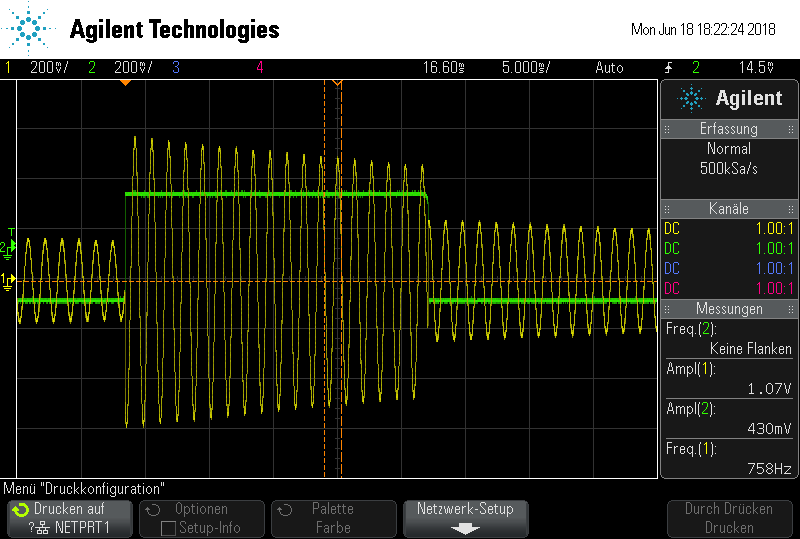
\includegraphics[width=\textwidth]{usb/scope_241.png}
	\caption{Die ungedämpfte Schwingung hat eine Frequenz von $f = \SI{758}{\hertz}$.}
	\label{scope_241}
\end{figure}
\begin{figure}[h]
	\centering
	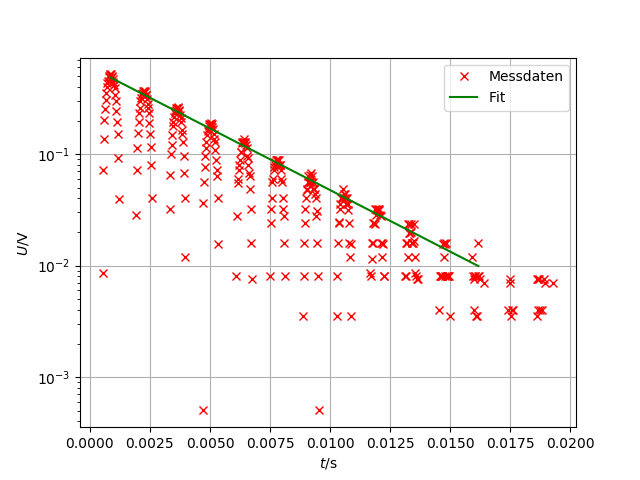
\includegraphics[width=\textwidth]{img/h.png}
	\caption{Die gedämpfte Schwingung klingt mit der Zeitkonstanten $\tau$ ab.}
	\label{h}
\end{figure}

\FloatBarrier
